\documentclass[tikz, border=10pt]{standalone}
\usepackage{iftex}
\ifluatex
  \usepackage{fontspec}
  \usepackage{unicode-math}
  \setmainfont{Fira Sans}
  \setmonofont{Fira Mono}
  \setmathfont{Fira Math}
\else
  \usepackage[T1]{fontenc}
\fi

\usepackage{pgfplots}
\pgfplotsset{compat=1.18}

% Theme toggle: \darkbgfalse for light background preview.
\newif\ifdarkbg
\darkbgtrue
\ifdarkbg
  \colorlet{axiscol}{white}
  \colorlet{gridcol}{white!30!black}
  \colorlet{ticklabelcol}{white}
  \colorlet{funcol}{lime!90!green}
  \colorlet{auxcol}{white!55!black}
\else
  \colorlet{axiscol}{black}
  \colorlet{gridcol}{black!25!white}
  \colorlet{ticklabelcol}{black}
  \colorlet{funcol}{blue!70!black}
  \colorlet{auxcol}{black!40!white}
\fi

\begin{document}
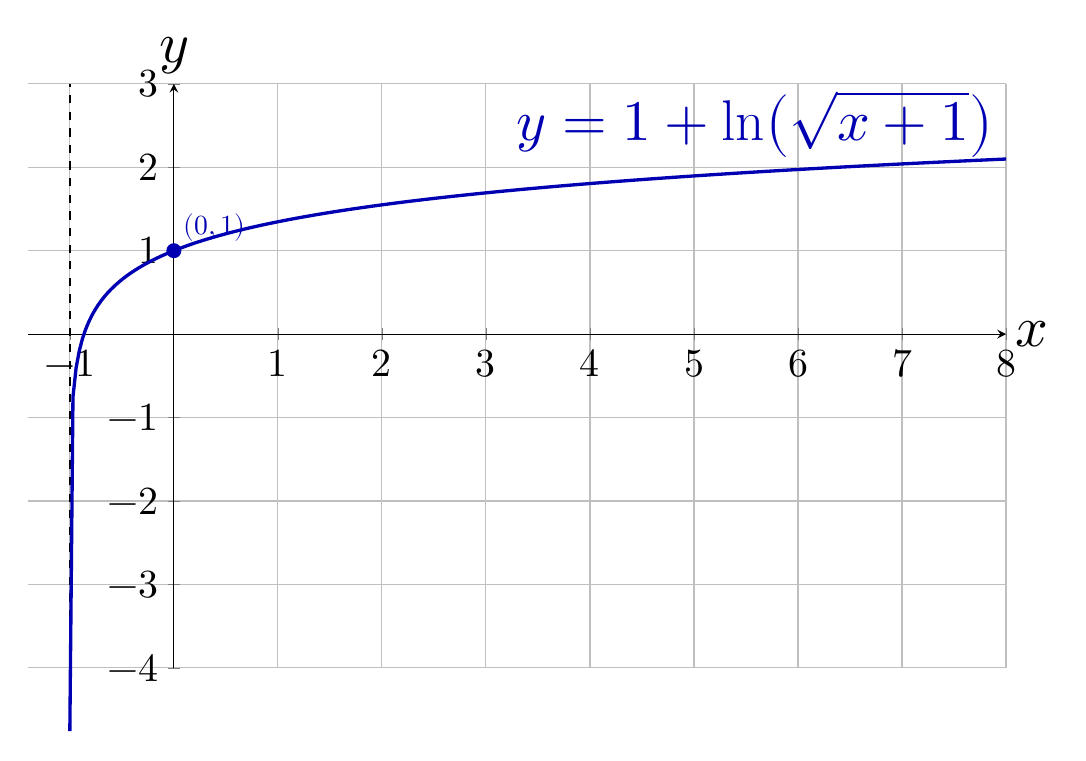
\begin{tikzpicture}
\begin{axis}[
  width=14cm,
  height=9cm,
  xmin=-1.4, xmax=8,
  ymin=-4, ymax=3,
  axis lines=center,
  axis line style={-stealth, thin, axiscol},
  grid=major,
  grid style={gridcol, thin},
  xtick={-1,0,1,2,3,4,5,6,7,8},
  ytick={-4,-3,-2,-1,0,1,2,3},
  xticklabel style={font=\Large, text=ticklabelcol},
  yticklabel style={font=\Large, text=ticklabelcol},
  xlabel={$x$},
  ylabel={$y$},
  xlabel style={at={(axis cs:8,0)}, anchor=west, text=axiscol, font=\huge},
  ylabel style={at={(axis cs:0,3)}, anchor=south, text=axiscol, font=\huge},
  clip=false,
]
  \addplot[dashed, thick, axiscol] coordinates {(-1,-4) (-1,3)};
  \addplot[very thick, funcol, domain=-0.99999:8, samples=300] {1 + ln(sqrt(x + 1))};
  \addplot[only marks, mark=*, mark size=2.5pt, funcol] coordinates {(0,1)};

%   \node[text=auxcol, anchor=south west] at (axis cs:-1,2.1) {$x=-1$};
  \node[text=funcol, anchor=west, font=\huge] at (axis cs:3.2,2.5) {$y=1+\ln\bigl(\sqrt{x+1}\bigr)$};
  \node[text=funcol, anchor=south west] at (axis cs:0,1) {$(0,1)$};
\end{axis}
\end{tikzpicture}
\end{document}